\subsection{Algoritmo genético}
Para esta práctica se desarrolló un algoritmo genético dicotómico que se apega al proceso mostrado en la Figura \ref{fig: AlgGenetico}

\begin{figure}[htbp]
	\centering
	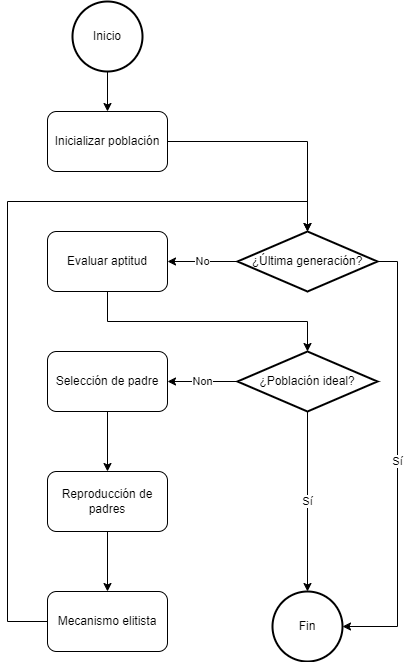
\includegraphics[width=0.5\textwidth]{algoritmo_genetico_proceso}
	\caption{Diagrama de flujo del algoritmo genético implementado.}
	\label{fig: AlgGenetico}
\end{figure}

Para llevar a cabo dicho proceso, se optó por utilizar el lenguaje de programación Python, donde se diseñaron métodos genéricos para realizar los procesos de generación de población, evaluación de aptitud, selección de individuos, reproducción de individuos y mecanismos elitistas.

\subsection{Implementación en Python}
\subsubsection{Inicializador de población}
\inputminted[linenos=true, fontsize=\scriptsize]{Python}{../../utils/population.py}

\subsubsection{Evaluación de individuos}
\inputminted[linenos=true, fontsize=\scriptsize]{Python}{../../utils/aptitude.py}

\subsubsection{Selección de parejas}
\inputminted[linenos=true, fontsize=\scriptsize]{Python}{../../utils/selection.py}

\subsubsection{Reproducción de individuos}
\inputminted[linenos=true, fontsize=\scriptsize]{Python}{../../utils/crossover.py}

\subsubsection{Mecanismo elitista}
\inputminted[linenos=true, fontsize=\scriptsize]{Python}{../../utils/elitist.py}

\subsubsection{Algoritmo completo}
\inputminted[linenos=true, fontsize=\scriptsize]{Python}{../demo.py}

\subsection{Pruebas realizadas}
Se implementaron un total de 2 mecanismos de selección, 2 mecanismos de cruza y 1 mecanismo elitista, por lo que se optó por realizar una combinación de todos los mecanismos diseñados para evaluar el desempeño de cada combinación. Las combinaciones resultantes fueron:

\begin{itemize}
	\item \textbf{Algoritmo 1.} Selección monogámica aleatoria + cruza de un punto.
	\item \textbf{Algoritmo 2.} Selección monogámica aleatoria + cruza de dos puntos.
	\item \textbf{Algoritmo 3.} Selección poligámica aleatoria + cruza de un punto.
	\item \textbf{Algoritmo 4.} Selección poligámica aleatoria + cruza de dos puntos.
\end{itemize}

Cabe destacar que, dado que solamente se implementó 1 mecanismo elitista, este fue aplicado a todos los algoritmos por igual. Además, para garantizar una comparación equitativa, se utilizó la misma población inicial para cada uno de los algoritmos.

Es importante mencionar que, para garantizar que el algoritmo se detuviera, se implementaron 2 criterios de paro:
\begin{itemize}
	\item \textbf{Número de generaciones.} Se estableció un límite de 10 generaciones para todos los algoritmos.
	\item \textbf{Término por $\epsilon$.} Se estableció un valor $\epsilon=0.8$ para determinar el fin del algoritmo.
\end{itemize}